%
% Documento: Disposições
%

\chapter{MATERIAIS E MÉTODOS}

\section{Materiais e ambiente de desenvolvimento}

O desenvolvimento do IncluiEdu envolveu duas configurações tecnológicas. Na etapa inicial, executada localmente, foram utilizados Python e Django para a aplicação, SQLite para armazenamento e Ollama para integração com inteligência artificial. Posteriormente, a versão atual passou a utilizar JavaScript e TypeScript, com backend em Cloudflare Workers, banco relacional Cloudflare D1 e geração de atividades por meio do Workers AI, com o modelo Gemma \cite{cloudflare2026workersai,cloudflare2026gemma,cloudflare2026d1}.

A interface web utiliza HTML, CSS e JavaScript para apresentar os recursos ao professor e comunicar-se com a API por requisições HTTP e dados em JSON. Na arquitetura atual, o arquivo \texttt{wrangler.jsonc} concentra a configuração do Worker, os vínculos com o banco de dados, o serviço de IA e os arquivos da interface. O código do projeto é mantido no GitHub.

A arquitetura atual utiliza serviços da Cloudflare para executar o backend, armazenar os registros e integrar a geração de atividades com inteligência artificial. O Cloudflare Workers processa as requisições da aplicação, o Cloudflare D1 mantém os dados relacionais e o Workers AI disponibiliza o modelo Gemma para a elaboração das propostas pedagógicas \cite{cloudflare2026workersai,cloudflare2026gemma,cloudflare2026d1}.

\section{Metodologia de desenvolvimento}

O desenvolvimento do IncluiEdu foi organizado em etapas, iniciadas pela definição das funcionalidades pedagógicas e pela modelagem das informações. Na primeira fase, a aplicação foi executada localmente com Django, SQLite e Ollama. Posteriormente, foi desenvolvida a versão atual, publicada na Cloudflare, com JavaScript, TypeScript, D1 e Workers AI. Ao longo do desenvolvimento, foram realizadas verificações manuais das funcionalidades.

A definição das funcionalidades considerou a necessidade de organizar turmas e alunos, registrar observações pedagógicas e apoiar o professor na elaboração de atividades personalizadas. Após a definição dos requisitos, foram elaborados modelos do sistema e implementados os recursos de autenticação, controle de acesso, acompanhamento e integração com a IA. A validação foi conduzida por verificações manuais da aplicação.

\section{Requisitos do sistema}

Os requisitos funcionais foram definidos com foco nas ações do professor e na proteção dos registros pedagógicos, conforme o Quadro~\ref{qua:requisitos-funcionais}.

\begin{quadro}[htb]
\centering
\caption{Requisitos funcionais do sistema}
\label{qua:requisitos-funcionais}
\begin{tabular}{|l|p{10cm}|}
\hline
\textbf{ID} & \textbf{Requisito funcional} \\
\hline
RF01 & Criar conta de professor \\
\hline
RF02 & Autenticar o professor \\
\hline
RF03 & Cadastrar e selecionar turmas \\
\hline
RF04 & Cadastrar e pesquisar alunos \\
\hline
RF05 & Restringir o acesso aos registros do professor \\
\hline
RF06 & Registrar observações pedagógicas \\
\hline
RF07 & Consultar o histórico das observações \\
\hline
RF08 & Classificar a situação do aluno \\
\hline
RF09 & Gerar atividades com Inteligência Artificial \\
\hline
RF10 & Armazenar as atividades geradas como rascunho \\
\hline
RF11 & Permitir a revisão das atividades pelo professor \\
\hline
RF12 & Permitir que o professor solicite a geração de uma imagem para complementar uma atividade pedagógica produzida com Inteligência Artificial \\
\hline
RF13 & Permitir que o professor consulte as atividades salvas no acompanhamento individual do aluno \\
\hline
\end{tabular}
\fonte{Elaborado pelos autores (2026).}
\end{quadro}

Entre os aspectos não funcionais contemplados na arquitetura estão a autenticação dos professores, a proteção das senhas e o controle de acesso aos registros pedagógicos, conforme o Quadro~\ref{qua:requisitos-nao-funcionais}.

\begin{quadro}[htb]
\centering
\caption{Requisitos não funcionais do sistema}
\label{qua:requisitos-nao-funcionais}
\begin{tabular}{|l|p{10cm}|}
\hline
\textbf{ID} & \textbf{Requisito não funcional} \\
\hline
RNF01 & As senhas dos professores devem ser armazenadas de forma protegida, utilizando mecanismos criptográficos de derivação de senha \\
\hline
RNF02 & O sistema deve utilizar sessões autenticadas para identificar o professor \\
\hline
RNF03 & O backend deve verificar a autorização do professor antes de permitir acesso ou alteração de registros protegidos.\\
\hline
RNF04 & RNF04	A comunicação entre a interface e o backend deve utilizar requisições HTTP e dados estruturados em JSON.\\
\hline
\end{tabular}
\fonte{Elaborado pelos autores (2026).}
\end{quadro}

\section{Modelagem do Sistenma}

A modelagem do sistema representa as interações do professor com a plataforma e as entidades relacionadas ao acompanhamento pedagógico. Os diagramas de casos de uso e de classes apresentam, respectivamente, as funcionalidades disponíveis e a organização dos elementos do sistema.

\subsection{DIAGRAMA DE CASOS DE USO}

O diagrama de casos de uso apresenta as principais funcionalidades disponibilizadas ao professor no IncluiEdu, incluindo o gerenciamento de turmas e alunos, o acompanhamento pedagógico, o registro de observações e a geração de atividades com Inteligência Artificial, conforme a Figura~\ref{fig:caso_de_uso}.

\begin{figure}[H]
    \centering
    \caption{Diagrama de Casos de Uso - IncluiEdu}
    \label{fig:caso_de_uso}
    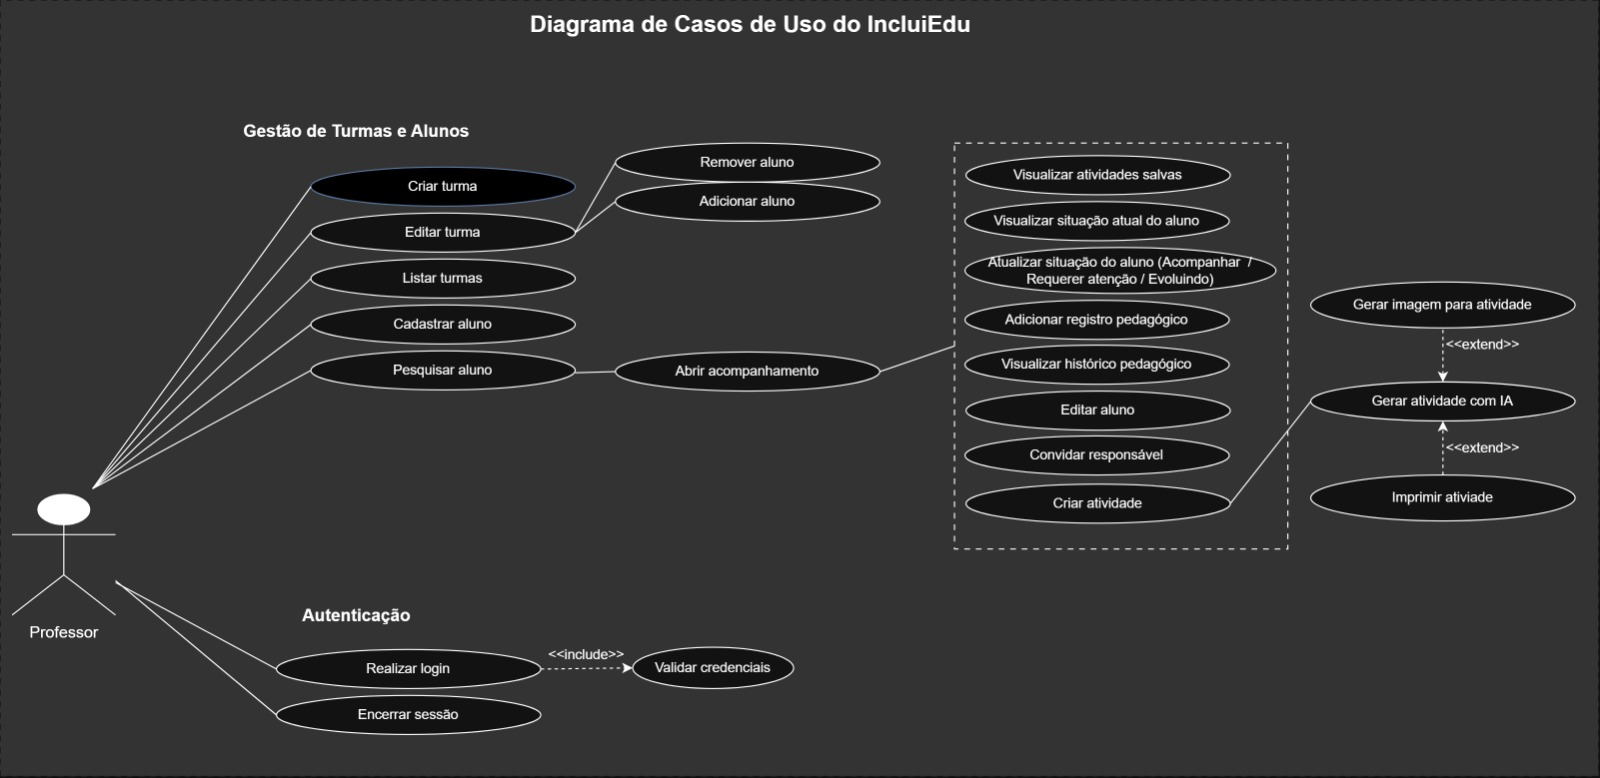
\includegraphics[width=0.9\textwidth]{04-figuras/casos_de_uso.jpeg}
    \fonte{Elaborado pelos autores (2026).}
\end{figure}

\subsection{DIAGRAMA DE CLASSES}
O diagrama de classes representa as principais entidades do sistema e seus relacionamentos. O professor está associado às turmas, que possuem alunos cadastrados. Cada aluno pode apresentar registros pedagógicos e atividades, permitindo a organização e a consulta das informações utilizadas no acompanhamento individual, conforme a Figura~\ref{fig:diagrama-classes}.

\begin{figure}[H]
    \centering
    \caption{Diagrama de Classes - IncluiEdu}
    \label{fig:diagrama-classes}
    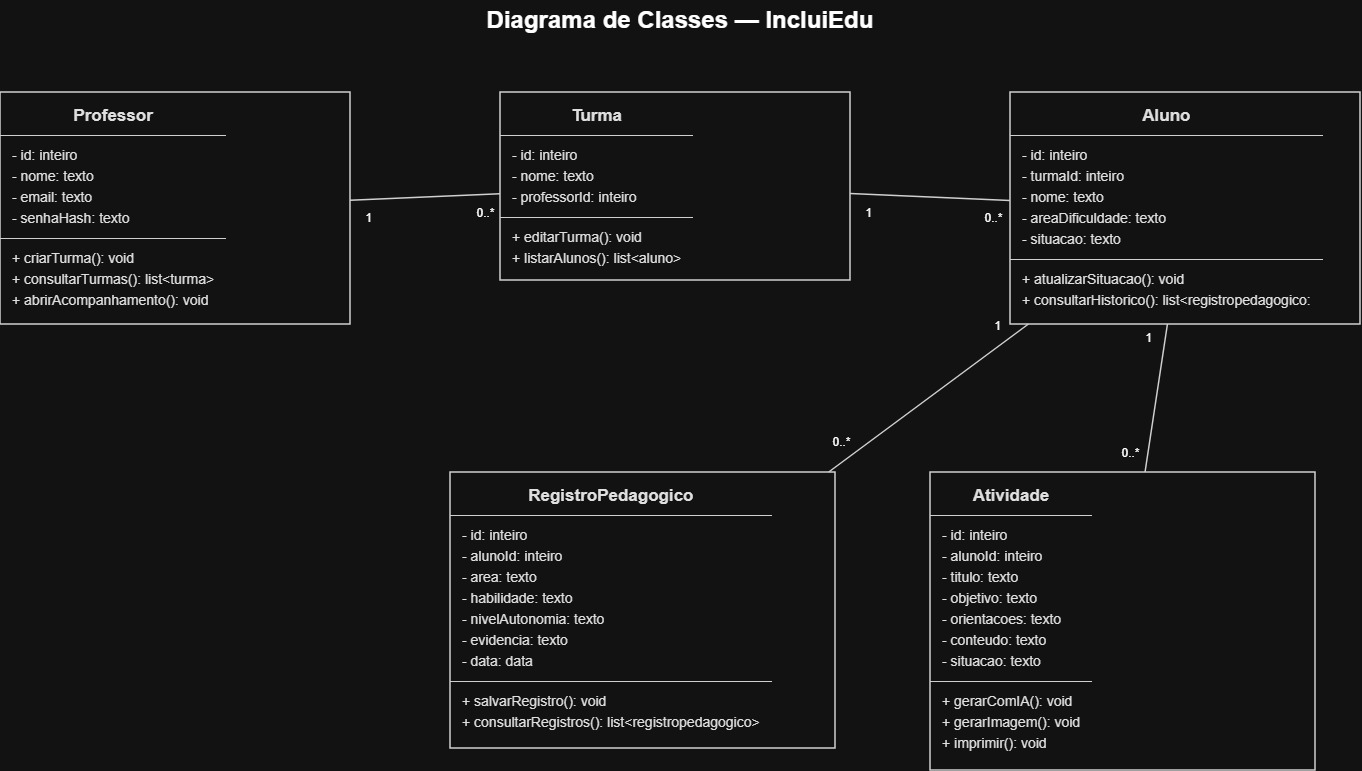
\includegraphics[width=0.9\textwidth]{04-figuras/diagrama_classes.jpeg}
    \fonte{Elaborado pelos autores (2026).}
\end{figure}

\subsection{MODELAGEM E IMPLEMENTAÇÃO DO BANCO DE DADOS}

A etapa local utilizou SQLite. Na versão atual, o Cloudflare D1 armazena dados em estrutura relacional \cite{cloudflare2026d1}. O modelo descrito compreende as entidades \texttt{users}, \texttt{classes}, \texttt{students}, \texttt{observations} e \texttt{activities}, relacionadas por chaves primárias e estrangeiras.

Um professor pode possuir diversas turmas; uma turma, diversos alunos; e cada aluno pode reunir observações e atividades ao longo do acompanhamento.

A estrutura do D1 é criada por migrações SQL, que documentam as tabelas e seus relacionamentos. As operações do backend utilizam instruções preparadas com parâmetros vinculados pelo método \texttt{.bind()}, evitando a concatenação direta dos valores recebidos em comandos SQL. O sistema verifica a vinculação dos registros ao professor autenticado antes de consultas ou alterações protegidas.

\begin{figure}[H]
    \centering
    \caption{Modelo do Banco de Dados - IncluiEdu}
    \label{fig:modelo-relacional}
    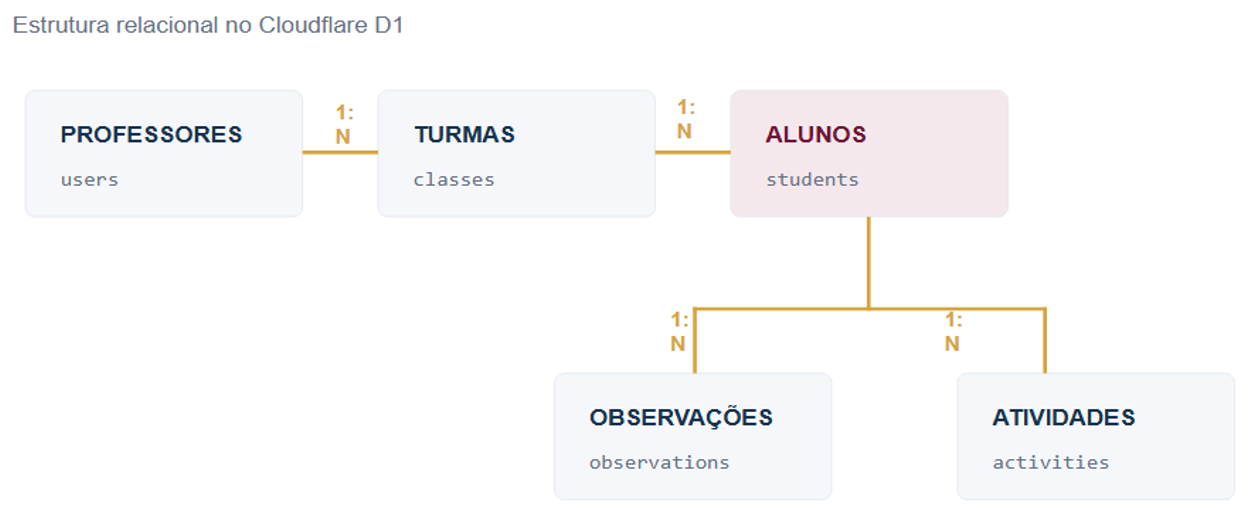
\includegraphics[width=0.9\textwidth]{04-figuras/modelo-relacional.png}
    \fonte{Elaborado pelos autores (2026).}
\end{figure}

\section{IMPLEMENTAÇÃO DO SISTEMA}

Na versão atual do IncluiEdu, a interface web apresenta as telas de cadastro, consulta e acompanhamento dos alunos. As ações realizadas pelo professor são enviadas à API por meio de requisições \texttt{fetch}, utilizando dados em formato JSON. O Cloudflare Worker recebe essas requisições, verifica a sessão e as permissões do usuário e realiza as operações necessárias no banco de dados D1. Em seguida, a resposta é enviada à interface, permitindo a atualização das informações apresentadas.

A autenticação utiliza derivação de senhas com PBKDF2, salt e SHA-256, evitando o armazenamento das senhas em texto simples. Após o login, o sistema cria uma sessão identificada por um cookie configurado com os atributos \texttt{HttpOnly}, \texttt{Secure} e \texttt{SameSite=Strict}. O backend também verifica se os registros acessados pertencem ao professor autenticado antes de permitir consultas ou alterações.

No acompanhamento pedagógico, cada registro reúne informações sobre o aluno, a área acompanhada, a habilidade observada, o nível de autonomia e as evidências registradas pelo professor. Esses dados são preservados no histórico pedagógico, permitindo acompanhar as observações realizadas ao longo do tempo. A situação do aluno também pode ser atualizada entre as opções \textit{Acompanhar}, \textit{Requer atenção} e \textit{Evoluindo}.

\section{TESTES E VALIDAÇÃO}

A verificação das funcionalidades do IncluiEdu foi realizada manualmente, por meio da interação com a aplicação. Os cenários de teste abrangem autenticação, organização de turmas, cadastro e consulta de alunos, observações pedagógicas, atualização da situação do aluno, geração de atividades e controle de acesso. Os procedimentos estão relacionados aos requisitos funcionais do sistema, conforme o Quadro~\ref{qua:testes}.

\begin{quadro}[htb]
\centering
\caption{Cenários de teste e resultados observados}
\label{qua:testes}
\small
\begin{tabular}{|p{2.5cm}|p{6cm}|p{5.5cm}|}
\hline
\textbf{Cenário} & \textbf{Procedimento realizado} & \textbf{Resultado} \\
\hline
Autenticação & Realização de login com credenciais válidas e inválidas. & O sistema permitiu o acesso com credenciais válidas e impediu a entrada com dados incorretos. \\
\hline
Turmas e alunos & Cadastro de turma e aluno, seleção de turma e pesquisa de aluno pelo nome. & As informações cadastradas foram exibidas corretamente, permitindo selecionar turmas e localizar alunos. \\
\hline
Acompanhamento & Abertura do acompanhamento individual de um aluno. & O sistema apresentou as informações do aluno, incluindo sua situação atual, registros pedagógicos e atividades salvas. \\
\hline
Registro pedagógico & Preenchimento dos campos de área, habilidade, nível de autonomia e evidência observada, seguido do salvamento. & O registro foi armazenado e disponibilizado para consulta no histórico pedagógico do aluno. \\
\hline
Situação do aluno & Alteração da situação entre \textit{Acompanhar}, \textit{Requer atenção} e \textit{Evoluindo}. & A situação foi atualizada e apresentada no perfil do aluno e no painel de acompanhamento. \\
\hline
Inteligência Artificial & Solicitação de uma atividade pedagógica personalizada por meio da IA. & O sistema apresentou uma atividade contendo título, objetivo, orientações e conteúdo pedagógico, identificada como rascunho para revisão. \\
\hline
Geração de imagem & Utilização da opção de gerar imagem para uma atividade produzida pela IA. & O sistema gerou uma imagem relacionada à atividade pedagógica solicitada, disponibilizando o resultado para utilização pelo professor. \\
\hline
Encerramento de sessão & Utilização da opção \textit{Sair} após autenticação. & A sessão foi encerrada, retornando o usuário à área de autenticação. \\
\hline
Controle de acesso & Tentativa de consultar registros de outro professor utilizando uma conta diferente. & O sistema impediu o acesso aos registros vinculados ao outro professor. \\
\hline
\end{tabular}
\fonte{Elaborado pelos autores (2026).}
\end{quadro}

Os testes manuais foram direcionados à observação do comportamento da versão atual da plataforma. A avaliação considerou os fluxos de utilização do professor e a comunicação entre interface, backend e serviços integrados.

\section{IMPLANTAÇÃO E REPRODUTIBILIDADE}

O IncluiEdu encontra-se publicado na plataforma Cloudflare, permitindo o acesso à aplicação por meio de um navegador web. A configuração do ambiente é organizada no arquivo \texttt{wrangler.jsonc}, que estabelece os vínculos necessários para o funcionamento dos serviços utilizados.

O código-fonte do projeto é mantido em um repositório no GitHub. Para reproduzir a aplicação em outro ambiente, é necessário obter os arquivos do projeto, configurar os serviços da Cloudflare, preparar o banco de dados D1 e realizar a publicação da aplicação.